\documentclass[11pt]{article}
\usepackage[UTF8,fontset=fandol]{ctex}
\usepackage[a4paper,margin=2.4cm]{geometry}
\usepackage{amsmath,amssymb,booktabs}
\usepackage{graphicx}
\usepackage[round]{natbib}
\usepackage[hidelinks]{hyperref}
\linespread{1.22}
\newcommand{\yes}{$\checkmark$}
\newcommand{\no}{--}
% Generated by reproduce.py. Edit the renderer or source data.
\newcommand{\FactorialRows}{%
A00 & 0 & 68.3 & 66.7 & $1.7\;[-3.3,7.0]$ \\
A00 & 1 & 60.0 & 65.0 & $-5.0\;[-15.3,6.7]$ \\
A00 & 2 & 65.0 & 61.7 & $3.3\;[0.0,10.3]$ \\
A01 & 0 & 81.7 & 55.0 & $26.7\;[1.7,48.4]$ \\
A01 & 1 & 90.0 & 61.7 & $28.3\;[9.8,48.3]$ \\
A01 & 2 & 78.3 & 45.0 & $33.3\;[11.7,54.8]$ \\
A10 & 0 & 68.3 & 30.0 & $38.3\;[15.8,57.4]$ \\
A10 & 1 & 60.0 & 36.7 & $23.3\;[6.9,38.3]$ \\
A10 & 2 & 65.0 & 40.0 & $25.0\;[3.4,43.5]$ \\
A11 & 0 & 81.7 & 41.7 & $40.0\;[16.7,62.7]$ \\
A11 & 1 & 90.0 & 28.3 & $61.7\;[38.3,83.1]$ \\
A11 & 2 & 78.3 & 38.3 & $40.0\;[20.3,58.7]$ \\
}
\newcommand{\SequenceRows}{%
A00 & 0 & 42 & 64.3 / 64.3 & 64.3 / 64.3 & 0.0 & 0.0 & 0.0 \\
A00 & 1 & 42 & 52.4 / 59.5 & 52.4 / 59.5 & -7.1 & -7.1 & -7.1 \\
A00 & 2 & 41 & 61.0 / 56.1 & 61.0 / 56.1 & 4.9 & 4.9 & 4.9 \\
A11 & 0 & 46 & 76.1 / 30.4 & 80.4 / 32.6 & 45.7 & 47.8 & 50.0 \\
A11 & 1 & 46 & 87.0 / 21.7 & 73.9 / 30.4 & 65.2 & 43.5 & 50.0 \\
A11 & 2 & 46 & 71.7 / 28.3 & 71.7 / 19.6 & 43.5 & 52.2 & 63.0 \\
}
\newcommand{\MainContrastRows}{%
0 & $45.7\;[17.2,72.1]$ & $47.8\;[26.5,69.7]$ & $50.0\;[27.9,71.8]$ \\
1 & $72.4\;[47.2,96.8]$ & $50.6\;[28.7,73.2]$ & $57.1\;[32.0,82.1]$ \\
2 & $38.6\;[14.4,61.7]$ & $47.3\;[20.3,72.3]$ & $58.2\;[28.3,84.1]$ \\
}
\newcommand{\AffineControlRows}{%
0 & $6.90\;[3.56,10.10]$ & $6.90\;[5.50,8.32]$ & 8.74 & 8.58 & 6.76 & 34/45 \\
1 & $8.16\;[4.36,11.58]$ & $8.16\;[6.65,9.70]$ & 9.11 & 9.07 & 7.45 & 35/46 \\
2 & $8.54\;[5.33,11.61]$ & $8.54\;[7.05,10.05]$ & 9.89 & 9.68 & 7.82 & 34/46 \\
}
\newcommand{\KDRows}{%
0 & 81.7 & 70.0 & $11.7\;[-1.6,25.4]$ & 15.2 & $6.39\;[3.65,8.81]$ \\
1 & 90.0 & 73.3 & $16.7\;[1.6,37.9]$ & 21.7 & $6.48\;[3.90,8.80]$ \\
2 & 78.3 & 76.7 & $1.7\;[-4.8,10.2]$ & 2.2 & $7.21\;[4.42,9.80]$ \\
}
\newcommand{\FactorialContrastRows}{%
A10$-$A00 & $36.7\;[15.5,54.8]$ & $28.3\;[13.8,42.4]$ & $21.7\;[0.0,41.3]$ \\
A11$-$A01 & $13.3\;[-1.6,30.0]$ & $33.3\;[10.0,55.2]$ & $6.7\;[-14.5,28.8]$ \\
A01$-$A00 & $25.0\;[-1.5,47.5]$ & $33.3\;[10.4,55.5]$ & $30.0\;[7.0,51.7]$ \\
A11$-$A10 & $1.7\;[-28.7,32.2]$ & $38.3\;[10.4,64.5]$ & $15.0\;[-13.2,44.0]$ \\
interaction & $-23.3\;[-47.6,3.4]$ & $5.0\;[-22.9,31.0]$ & $-15.0\;[-44.0,16.1]$ \\
}
\newcommand{\EqualFamilyRows}{%
A01$-$A00 & $23.2\;[-2.5,46.2]$ & $32.8\;[10.5,54.7]$ & $29.5\;[6.7,51.6]$ \\
A11$-$A10 & $1.1\;[-29.2,31.7]$ & $38.4\;[10.3,64.7]$ & $15.2\;[-12.7,43.8]$ \\
}
\newcommand{\ScoringChangeRows}{%
0 & $2.2\;[-25.5,25.0]$ & $2.2\;[-25.5,25.0]$ & $2.2\;[-17.4,21.7]$ & $3.6\;[-24.4,26.2]$ \\
1 & $-21.7\;[-34.0,-13.0]$ & $-21.7\;[-38.9,-5.2]$ & $-21.7\;[-39.5,-4.1]$ & $-20.8\;[-37.8,-5.1]$ \\
2 & $8.7\;[-10.9,30.4]$ & $8.7\;[-10.6,30.4]$ & $8.7\;[-6.5,23.9]$ & $9.2\;[-10.7,31.5]$ \\
}
\newcommand{\AllPairsRows}{%
A00 & 0 & 1.7 & 0.0 & 0.0 \\
A00 & 1 & -5.0 & -5.0 & -5.0 \\
A00 & 2 & 3.3 & 3.3 & 3.3 \\
A11 & 0 & 40.0 & 43.3 & 45.0 \\
A11 & 1 & 61.7 & 40.0 & 45.0 \\
A11 & 2 & 40.0 & 46.7 & 55.0 \\
}

% Generated by scripts.reanalysis_tables.py from reports/audit_reanalysis.json.
\newcommand{\ControlTestRows}{%
0 & mismatch & -1.89\,[-2.89,-0.89] & 0.009 & 0.419 & \no \\
0 & zero & -1.71\,[-2.63,-0.79] & 0.010 & 0.285 & \no \\
0 & random & 0.01\,[-2.15,2.17] & 0.993 & 0.062 & \no \\
1 & mismatch & -0.93\,[-1.75,-0.12] & 0.067 & 0.021 & \yes \\
1 & zero & -0.88\,[-1.64,-0.11] & 0.068 & 0.014 & \yes \\
1 & random & 0.67\,[-0.60,1.95] & 0.352 & 0.045 & \yes \\
2 & mismatch & -1.30\,[-2.35,-0.25] & 0.052 & 0.123 & \no \\
2 & zero & -1.09\,[-2.25,0.07] & 0.119 & 0.091 & \no \\
2 & random & 0.72\,[-0.33,1.78] & 0.236 & 0.028 & \yes \\
}
\newcommand{\ControlMeanRows}{%
0 & mismatch & 8.74\,[5.04,12.16] & 6.90\,[3.56,10.10] \\
0 & zero & 8.58\,[4.62,12.11] & 6.90\,[3.56,10.10] \\
0 & random & 6.76\,[3.90,9.92] & 6.90\,[3.56,10.10] \\
1 & mismatch & 9.11\,[5.20,12.58] & 8.16\,[4.36,11.58] \\
1 & zero & 9.07\,[5.10,12.64] & 8.16\,[4.36,11.58] \\
1 & random & 7.45\,[4.26,10.50] & 8.16\,[4.36,11.58] \\
2 & mismatch & 9.89\,[5.99,13.49] & 8.54\,[5.33,11.61] \\
2 & zero & 9.68\,[5.64,13.35] & 8.54\,[5.33,11.61] \\
2 & random & 7.82\,[4.71,10.77] & 8.54\,[5.33,11.61] \\
}
\newcommand{\ScaleRows}{%
A00 & 0 & 6.16 & 1.97 & 0.32 \\
A00 & 1 & 5.90 & 1.93 & 0.33 \\
A00 & 2 & 6.64 & 2.12 & 0.32 \\
A11 & 0 & 8.62 & 6.90 & 0.80 \\
A11 & 1 & 9.08 & 8.16 & 0.90 \\
A11 & 2 & 9.71 & 8.54 & 0.88 \\
}
\newcommand{\RankRows}{%
affine & -0.436 & $<10^{-8}$ & 180 \\
kd & +0.435 & $<10^{-8}$ & 180 \\
}
\newcommand{\MapperGapRows}{%
0 & 6.90\,[3.56,10.10] & 6.39\,[3.65,8.81] & 0.417 & 0.700 \\
1 & 8.16\,[4.36,11.58] & 6.48\,[3.90,8.80] & 0.283 & 0.733 \\
2 & 8.54\,[5.33,11.61] & 7.21\,[4.42,9.80] & 0.383 & 0.767 \\
}
\newcommand{\ExtendedScoringRows}{%
A00 & 0 & 1.7\,[-3.3,7.0] & 0.0\,[-4.8,5.1] & 0.0\,[-4.8,5.1] \\
A11 & 0 & 40.0\,[16.7,62.7] & 43.3\,[24.2,62.1] & 45.0\,[25.8,63.3] \\
A00 & 1 & -5.0\,[-15.2,6.7] & -5.0\,[-11.9,0.0] & -5.0\,[-11.9,0.0] \\
A11 & 1 & 61.7\,[38.3,83.0] & 40.0\,[21.3,58.3] & 45.0\,[23.8,66.1] \\
A00 & 2 & 3.3\,[0.0,10.3] & 3.3\,[0.0,10.3] & 3.3\,[0.0,10.3] \\
A11 & 2 & 40.0\,[20.3,58.7] & 46.7\,[24.1,68.3] & 55.0\,[29.5,78.3] \\
}
\newcommand{\ExtendedContrastRows}{%
0 & 38.3\,[13.9,61.2] & 43.3\,[23.7,62.8] & 45.0\,[25.0,64.5] \\
1 & 66.7\,[40.8,90.2] & 45.0\,[25.3,64.0] & 50.0\,[27.9,71.1] \\
2 & 36.7\,[16.1,56.5] & 43.3\,[20.0,66.0] & 51.7\,[26.2,76.3] \\
}
\newcommand{\ScoringCountRows}{%
retained\_6\_family & A00 & 0 & 42 & 6 \\
retained\_6\_family & A00 & 1 & 42 & 6 \\
retained\_6\_family & A00 & 2 & 41 & 6 \\
retained\_6\_family & A11 & 0 & 46 & 6 \\
retained\_6\_family & A11 & 1 & 46 & 6 \\
retained\_6\_family & A11 & 2 & 46 & 6 \\
f1\_f4\_all\_6\_family & A00 & 0 & 46 & 6 \\
f1\_f4\_all\_6\_family & A00 & 1 & 46 & 6 \\
f1\_f4\_all\_6\_family & A00 & 2 & 46 & 6 \\
f1\_f4\_all\_6\_family & A11 & 0 & 46 & 6 \\
f1\_f4\_all\_6\_family & A11 & 1 & 46 & 6 \\
f1\_f4\_all\_6\_family & A11 & 2 & 46 & 6 \\
all\_60\_pairs\_8\_family & A00 & 0 & 60 & 8 \\
all\_60\_pairs\_8\_family & A00 & 1 & 60 & 8 \\
all\_60\_pairs\_8\_family & A00 & 2 & 60 & 8 \\
all\_60\_pairs\_8\_family & A11 & 0 & 60 & 8 \\
all\_60\_pairs\_8\_family & A11 & 1 & 60 & 8 \\
all\_60\_pairs\_8\_family & A11 & 2 & 60 & 8 \\
}


\title{基准重建如何反转一项跨模型 KV 迁移发现\\[2pt]
\large 受控版本对照、对照检验与指标诊断}
\author{Xuemin Zhang$^{1}$ \quad Liangbin Hu$^{1}$ \quad Kun Yi$^{1}$ \quad Liheng Zhong$^{1}$ \quad Junpeng Yu$^{1}$\\[2pt]
\small $^{1}$CETC}
\date{}

\begin{document}
\maketitle

\begin{abstract}
\noindent
跨模型键值（KV）缓存迁移通常在配对反事实基准上评估。我们审计了 Qwen3-1.7B$\to$0.6B 的一套此类基准，发现 18 个“必须翻转却候选相同”的退化配对、至少 15 组跨切分文档逐字重叠，以及校准集与留出集共享模板骨架。重建语料反转了仿射映射的表面成功：其“原生减迁移”双侧正确率差距在“原始/原始”条件下为 $-5.0$ 至 $3.3$ 个百分点，而在其余九个单元—种子组合中为 $23.3$ 至 $61.7$ 个百分点。在重建验证集上，迁移后的反事实误差不大于错配与置零缓存对照、接近随机缓存对照，且在一颗种子上显著小于置零对照，尽管双侧正确率同时坍塌到 $28.3\%$--$41.7\%$。预声明的等价性检验（$\delta=2$ 对数概率单位）只在三颗种子中的一颗成立，因此“与零信息对照无法区分”并未得到一致支持。我们进一步表明，反事实误差的区分效度很弱：它与一个双侧正确率相差 $28$--$45$ 个百分点的蒸馏基线之间的区间相互重叠，且其与正确率的秩相关在两个映射器之间反号。完整候选打分在每颗种子上都保住了版本对比的方向，但其中一颗的幅度下降了 $21.7$ 个百分点。所有估计均为探索性（至多八个模板族），只覆盖一个合成模型对，且不把反转归因于任何单一缺陷。单缺陷干预、封存测试与第二个模型对仍未评测。我们发布修复后的基准、数值账本与审计协议。
\end{abstract}

\noindent\textbf{关键词}：KV 缓存迁移；基准审计；数据泄漏；对照检验；指标效度；探索性区间

\section{引言}

缓存翻译让接收端模型复用另一个模型处理过的文档所产生的键值对，而不必再次预填该文档。下游答案正确率衡量传过去的缓存是否有用；配对文档设计还可以追问：文档中的事实被改动时，接收端的候选打分是否随之改变。这两个量可以给出相反的信号，而要诊断这种分歧，前提是文档对本身有效，且接收端在两种文档变体下都能作答。

我们此前在一套合成配对基准上的分析提示，仿射 KV 映射在保持双侧正确率的同时改变了反事实响应打分，并据此提出了一个接收端消费值的机制猜想。审计该基准后，我们撤回了这两项论断：遗留语料包含退化配对、跨切分文档重叠与重叠的模板骨架，而其不确定性估计实际上把相关样本当作独立样本。

\paragraph{本研究确立了什么。}
我们把一个模型对的原始与重建校准语料、验证语料交叉，得到十二个单元—种子组合。替换任一语料都把正确率差距从接近零推到 $23.3$--$61.7$ 个百分点。随后我们提出两个仅靠版本对照无法回答的问题：第一，在使用逐种子聚类区间与预声明的等价边界之后，迁移后的反事实误差与显式的无信息对照相比如何？第二，反事实误差是否真的能反映迁移是否有用？我们从归档打分回答这两个问题，不做新的模型运行。第三项检查追问：当对完整候选序列而不是只对首 token 打分时，方向是否保持。

\paragraph{贡献。}
(1) 一套缺陷分类与审计协议，覆盖退化配对、跨切分泄漏、实体与模板骨架重叠，以及聚类 bootstrap 退化。(2) 一个修复后的配对基准（\texttt{cf\_pairs\_v2.1}）及发布的数值账本与 CPU 回放。(3) 受控证据：正确率差距对语料版本敏感，并附带对照、等价性与指标效度诊断——反事实误差无法区分有用与无用的映射器，而双侧正确率可以。(4) 一项打分读出检查：方向保持而幅度不保持。

\paragraph{主张范围。}
这是一次对单一等深模型对、合成中文模板数据的审计，至多八个模板族，封存测试仍未评测。我们不把反转归因于任何单一缺陷，不声称在干净数据上存在某种机制，不声称跨模型或跨模型对的泛化，也不声称等价性检验有足够功效。失败的等价性检验按“不确定”报告，而不是当作“存在缺陷”的证据。所有估计自始至终都是探索性的。

\paragraph{相关工作。}
\citet{heo2026} 给出逐层闭式线性映射，并报告在某些模型对上退化明显；\citet{kvlingo} 用蒸馏训练 KV 翻译器；\citet{cachelink} 区分“重建保真度”与“接收端可用性”；\citet{cheng2026} 用错配、置零与随机缓存检验示例特定信息的作用。我们的对照设计与后者同源，但关注点是可复现的“基准版本反转”。最小改动输入的思路来自对比集评估 \citep{contrastsets}；数据审计针对的泄漏与相关评估单元问题见 \citet{kapoor2023}。本文的增量是校准$\times$验证的交叉比较，及其对照、指标与打分诊断。

\section{基准与审计}

\paragraph{配对文档任务。}
每个示例包含一个问题、两篇独立构造的文档、两个候选答案。四个语义切片要求“改动必须翻转正确答案”：直接事实替换（F1）、推理链（F2）、关系或否定改变（F3）、干扰项与共指（F4）。F5 的两个候选文本完全相同，用作“不应翻转”的对照；F6 只改人名及其答案标签，同时控制长度与位置。F6 单独报告，F5 与 F6 都不参与方向一致性分析。

\paragraph{重建做了什么。}
归档的 seed-0 语料共 520 对（校准 120、验证 60、探针 40、测试 300）。审计发现：18 个“必须翻转却候选相同”的退化配对、至少 15 组跨切分逐字重叠、校准与留出集共享实体与模板骨架，而历史重采样单元实质上就是单个配对。重建时我们让候选在需要翻转处真正不同、把实体池按切分隔离、去重、并在探针与留出集引入结构上未见过的模板。就本文使用的验证集而言，每版本每颗种子有 46 对落在 F1--F4；原始验证集的退化配对数为 $4,4,5$，校准与验证之间逐字相同的文档串为 $2,5,1$；重建后两者均为零。重建语料中 F1--F4 共有 398 个示例（全语料计数）。图~\ref{fig:corpus} 给出这三个缺陷在重建前后的对照。

\begin{figure}[tbp]
\centering
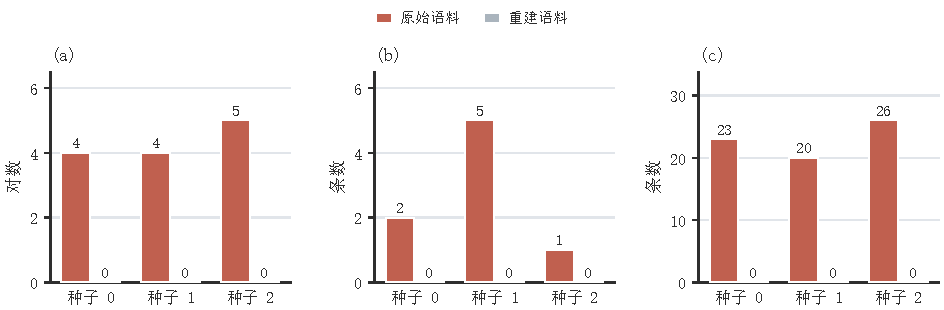
\includegraphics[width=\linewidth]{figures/fig2_corpus_zh.pdf}
\caption{重建前后验证集上的缺陷计数（由随包语料文件重算）。(a) F1--F4 中两个候选完全相同、却要求翻转的配对；(b) 校准与验证之间逐字相同的文档串；(c) 两套切分之间重复的查询串。三种缺陷在重建语料上均为零；各面板纵轴刻度独立。}
\label{fig:corpus}
\end{figure}

\paragraph{一句警告。}
我们把语料版本当作“整包”比较：一次替换同时改变了候选、实体池、模板与去重状态。因此本文能说“换成这一包语料后结果变了”，不能说“变化来自其中某一个缺陷”。校准集影响映射本身，验证集影响被测量的任务与原生参照，两者在原理上可分离，所以才有下面的 $2\times2$ 交叉。计划中的封存测试方法终点仍未评测，单缺陷干预也尚未运行。

\section{评估}

\paragraph{模型、映射与两种缓存条件。}
发送端 Qwen3-1.7B、接收端 Qwen3-0.6B，均为 28 层且逐层对应；接收端权重全程冻结。仿射映射对每一层、每个头、K 与 V 分别拟合岭回归，用 120 对校准样本的配对缓存作训练，$\lambda=10^{-3}$，闭式解，含截距约 $7.40\times10^{6}$ 个系数。归档 GPU 运行使用 bfloat16 与 SDPA。

\emph{Self} 条件使用接收端自己对同一文档的原生缓存；\emph{Joint} 条件把发送端的键与值都映射后注入。接收端只看到查询与（整串打分时的）候选前缀，文档位置来自注入缓存。恒等注入用于检查接收端的缓存通路：在 80 个文档侧上的初步诊断显示原生缓存与恒等注入一致，报告的最小余弦值四舍五入为 $1.0$，首 token KL 为零。此外还有三种对照缓存——错配（同一验证集内确定性的“下一示例”替换）、置零、随机——用来给出“迁移误差”的量级参照；错配对照采用上述实验中的取值，因为历史上的错配选择方式不同。

\paragraph{两种候选打分。}
记 $s(c;C,q)$ 为候选 $c$ 在查询 $q$、缓存 $C$ 下的得分。首 token 口径取候选首 token 的下一 token 对数概率；复核口径取教师强制下全部候选 token 的条件对数概率之和，并另做长度归一。候选从各自独立初始化的接收端缓存分支出发，查询与候选分别分词后拼接、不加 EOS。两种口径都按候选在两侧文档上分别排序，同分时沿用历史规则（先到者胜），且“两个候选都判对”时记为该对正确。用这套规则在 CPU 上回放，720 条首 token 双侧标签全部与归档一致。需要说明的是，统一口径之前，序列评分入口在 F5 上无法识别“任一候选即可”的金标签，造成 84 条标签不同；在语义样本上把同分判给第二个候选，造成 6 条标签不同；统一口径后这一差异消失。

\paragraph{指标。}
分别报告 Self 与 Joint 的“双侧同时正确”比例，记 $L$ 为两者之差（百分点）：

\begin{align}
g(C,q) &= s(A;C,q)-s(B;C,q),\\
D &= g(C(d_A),q)-g(C(d_B),q),\\
E_{\mathrm{CF}} &= \left| D_{\mathrm{Joint}}-D_{\mathrm{Self}} \right|.
\end{align}

$E_{\mathrm{CF}}$ 是 Joint 相对 Self 的反事实偏差，按定义 Self 相对自身为零。不同打分口径给出不同的误差尺度，因此只在同一口径内比较误差，跨口径只比较正确率。方向一致性统计 F1--F4 中 $|D_{\mathrm{Self}}|>0.1$ 的配对，其 Joint 与 Self 的 $D$ 同号的比例，并给出分子与分母。

\paragraph{设计与区间。}
校准集合取\{原始,\,重建\}、验证集合取\{原始,\,重建\}，两者交叉成四个单元：A00 为“原始/原始”（历史配置），A01 换验证、A10 换校准、A11 两者都换。每单元三颗独立数据种子，每格 60 对验证样本。固定验证集的比较按样本配对；跨验证集的比较对两套样本独立重采样。区间由模板族（每版本 8 族，语义子集 6 族）重采样 10000 次得到，区间宽度是样本加权口径；族等权的点估计与区间作为敏感性另附。所有区间均为探索性 95\% 百分位区间，种子逐个报告而不取平均。语料版本设计在正式运行前已定稿；整串打分的方案在可复现重跑之前已提交版本库，早于它的工程性试跑仍留在档案里，但不用于主效应估计。对照比较的等价边界 $\delta=2$ 在查看本修订版的数字之前已写入 \texttt{configs/prereg/equivalence\_margin\_v2.9.yaml}；它是内部版本控制的协议，而非外部注册。图~\ref{fig:design} 画出这条路径与四个单元。

\begin{figure}[tbp]
\centering
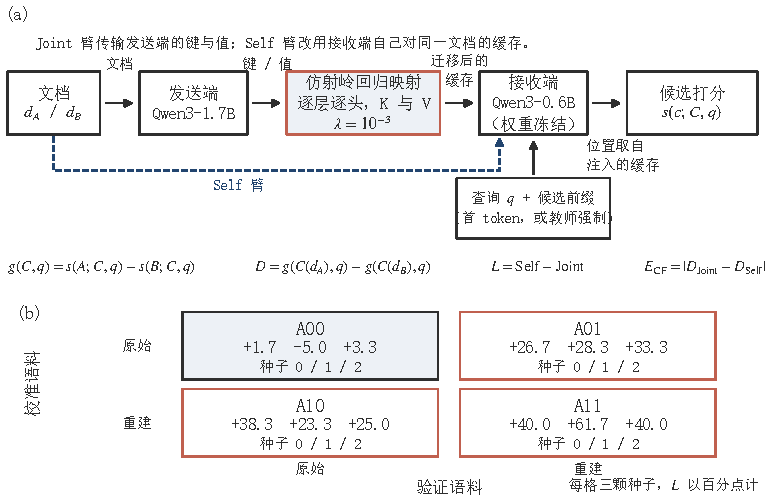
\includegraphics[width=\linewidth]{figures/fig1_design_zh.pdf}
\caption{缓存路径与语料版本设计。(a) 发送端逐层的键与值经逐层逐头的仿射岭回归映射后注入冻结的接收端，接收端只看查询与候选前缀；Self 臂改用接收端自己对同一文档的缓存。(b) 原始（0）与重建（1）的校准、验证语料交叉，每格三颗种子，格内标注三种子的 $L$（百分点），历史对角格加灰底。$g$、$D$、$L$、$E_{\mathrm{CF}}$ 的定义见第 3 节。}
\label{fig:design}
\end{figure}

\section{结果}

\subsection{校准集与验证集版本都会改变结果}

\begin{table}[tbp]
\centering
\caption{语料版本比较：每单元每颗种子 60 对验证样本。Self 与 Joint 为双侧正确率（\%），$L$ 及其模板族区间以百分点计。}
\label{tab:factorial}
\small
\begin{tabular}{lrrrr}
\toprule
单元 & 种子 & Self & Joint & $L$ [95\% 区间]\\
\midrule
\FactorialRows
\bottomrule
\end{tabular}
\end{table}

表~\ref{tab:factorial} 与图~\ref{fig:factorial} 给出同一批数字的两种读法。历史对角格 A00 的三颗种子分别为 $1.7$、$-5.0$、$3.3$ 个百分点，族区间都与零重叠；其余九个单元在 $23.3$ 至 $61.7$ 个百分点之间，区间基本离开零。固定验证集、只换校准语料时，$L$ 分别上升 $36.7$、$28.3$、$21.7$ 个百分点（验证集为原始）；换成重建验证集后，相应上升为 $13.3$、$33.3$、$6.7$。

换验证集同样会移动参照。以种子 0、校准集为重建为例：Joint 从 $30.0\%$ 升到 $41.7\%$，Self 同时从 $68.3\%$ 升到 $81.7\%$，于是差距反而扩大 $1.7$ 个百分点——迁移确实变好了，但原生参照升得更快。两个固定验证集的校准对比之差（即交互项）在三颗种子上分别为 $-23.3$、$5.0$、$-15.0$ 个百分点，探索性区间都覆盖零；也就是说，本文能确认“每一处切换都改变了结论”，但不能确认交互的方向。把分析限制在语义切片、或剔除候选相同的对照样本，A00 与其余单元的对比关系不变。

\begin{figure}[tbp]
\centering
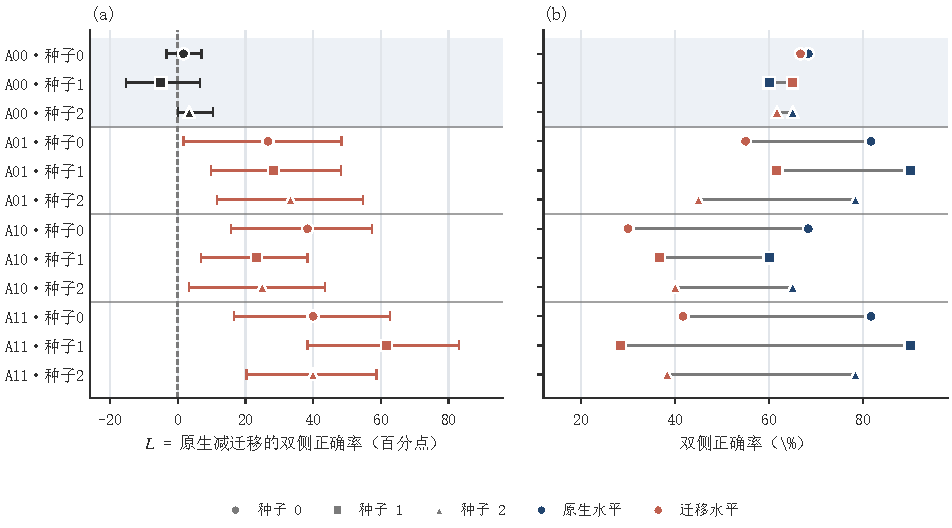
\includegraphics[width=\linewidth]{figures/fig3_factorial_zh.pdf}
\caption{语料版本结果。(a) 每个单元每颗种子的 $L$ 及其模板族区间，历史对角格 A00 以灰底标出，虚线为零差距参考。(b) 产生该差距的两个正确率水平：左端为迁移、右端为原生，同一行内比较才成立。}
\label{fig:factorial}
\end{figure}

\subsection{反事实误差与无信息对照}

在重建的校准集与验证集上，Joint 的首 token 反事实误差在三颗种子上分别为 $6.90$、$8.16$、$8.54$，族区间见表~\ref{tab:control-test}。每个值都不大于对应的错配、置零与随机缓存均值；配对族层面的差值在错配与置零上所有种子都为负，其中对置零对照的种子 0 达到双侧 $p=0.010$，种子 1 为 $p=0.068$。因此方向在一颗种子上具有统计可辨性，这与简单的“无信息”解读相反。

\begin{table}[tbp]
\centering
\caption{重建验证集上 Joint 减对照的反事实误差。差值与 90\% 族 $t$ 区间以对数概率单位计；$p_2$ 为八个族均值的双侧配对 $t$ 检验；TOST 使用预声明的 $\delta=2$；$\checkmark$ 表示等价成立。}
\label{tab:control-test}
\begin{tabular}{lrrrrr}
\toprule
种子 & 对照 & Joint $-$ 对照 [90\% CI] & $p_2$ & TOST $p$ & 等价\\
\midrule
\ControlTestRows
\bottomrule
\end{tabular}
\end{table}

预声明的等价性检验并非一致成立：在 $\delta=2$ 下，它只在种子 1 对三种对照都成立，并在种子 2 对随机对照成立，但在种子 0 和 2 对错配或置零对照都不成立。种子 0 的点估计落在边界之内，但其区间下沿低于 $-2$。因此我们只报告有支持的陈述：Joint 的误差不大于错配与置零对照、接近随机对照，且在一颗种子上显著小于置零对照，而其双侧正确率同时跌到 $28.3\%$--$41.7\%$。两件事合在一起，是度量本身可被诊断出的不一致，而不是“迁移保住了效用”的证据。各对照均值及其区间见附录表~\ref{tab:control-mean}。图~\ref{fig:controls} 把误差与三种对照、以及逐配对的符号关系画在一起。

\begin{figure}[tbp]
\centering
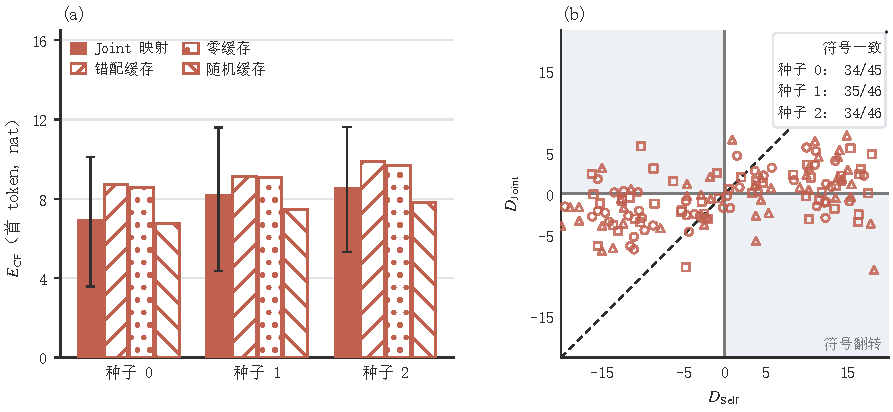
\includegraphics[width=\linewidth]{figures/fig5_controls_zh.pdf}
\caption{反事实误差与对照缓存。(a) 仿射映射的首 token $E_{\mathrm{CF}}$ 与错配、置零、随机三种对照缓存的均值；误差棒为 Joint 臂的模板族区间。(b) 语义切片上逐配对的 $D_{\mathrm{Self}}$ 与 $D_{\mathrm{Joint}}$；靠近对角线的点两侧同号，左上与右下为符号翻转区，$|D|>20$ nat 的点不绘出，内嵌为每个种子的同号分子/分母。}
\label{fig:controls}
\end{figure}

\subsection{反事实误差测量的是什么}

重建后 $E_{\mathrm{CF}}$ 上升约四倍，并不只是 Self 参照的量纲变化。平均 $|D_{\mathrm{Self}}|$ 从 A00 的 $5.90$--$6.64$ 升到 A11 的 $8.62$--$9.71$，约 $1.4$ 倍；而平均 Joint $E_{\mathrm{CF}}$ 从 $1.93$--$2.12$ 升到 $6.90$--$8.54$，约 $3.5$--$4$ 倍（表~\ref{tab:scale}）。用 $|D_{\mathrm{Self}}|$ 归一化后，比值仍从约 $0.32$ 升到 $0.80$--$0.90$。

\begin{table}[tbp]
\centering
\caption{Self 参照与 Joint 误差的尺度。$E_{\mathrm{CF}}/|D_{\mathrm{Self}}|$ 使用逐种子均值；所有量均以对数概率单位计。}
\label{tab:scale}
\begin{tabular}{lrrrr}
\toprule
单元 & 种子 & mean $|D_{\mathrm{Self}}|$ & mean Joint $E_{\mathrm{CF}}$ & 比值\\
\midrule
\ScaleRows
\bottomrule
\end{tabular}
\end{table}

更重要的是，$E_{\mathrm{CF}}$ 并不按可用性给映射器排序。在每个映射器 180 对重建验证配对上，双侧正确率与 $E_{\mathrm{CF}}$ 的 Spearman 相关在仿射映射为 $-0.436$，在蒸馏基线为 $+0.435$（附录表~\ref{tab:rank}），符号反转。两者的 $E_{\mathrm{CF}}$ 族区间在每颗种子都相互重叠，而双侧正确率相差 $28$--$45$ 个百分点（附录表~\ref{tab:mapper-gap}）。较低的反事实误差可以伴随坍塌的双侧正确率，较高的也可以伴随保持的正确率。因此我们把 $E_{\mathrm{CF}}$ 当作打分差异的诊断量，而把并列报告的 Self 与 Joint 正确率当作可解释的终点。

\begin{figure}[tbp]
\centering
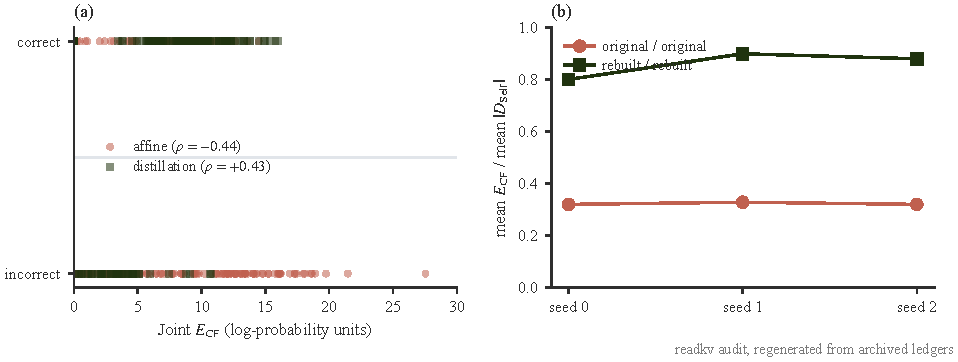
\includegraphics[width=\linewidth]{figures/fig7_ecf_zh.pdf}
\caption{反事实误差的诊断。(a) 重建验证集上两个映射器各 180 对配对的 Joint 双侧正确率对首 token $E_{\mathrm{CF}}$；秩相关的符号在两者之间反转。(b) 平均 $E_{\mathrm{CF}}$ 除以平均 $|D_{\mathrm{Self}}|$：重建单元并不只是原始单元的重新缩放。}
\label{fig:ecf}
\end{figure}

\subsection{整串打分保住方向，但幅度会动}

\begin{table}[tbp]
\centering
\caption{打分复核（语义子集，候选相异且金标签互换）。“原生/迁移”为 Self/Joint 的双侧正确率（\%）；末三列为 $L$（百分点）。}
\label{tab:sequence}
\small
\begin{tabular}{lrrrrrrr}
\toprule
& & & \multicolumn{2}{c}{原生 / 迁移} & \multicolumn{3}{c}{$L$（百分点）}\\
\cmidrule(lr){4-5}\cmidrule(l){6-8}
单元 & 种子 & 对子数 & 首 token & 整串 & 首 token & 整串 & 归一\\
\midrule
\SequenceRows
\bottomrule
\end{tabular}
\end{table}

\begin{table}[tbp]
\centering
\caption{每种打分口径下的版本差 $L_{\mathrm{A11}}-L_{\mathrm{A00}}$，数值与探索性模板族区间均以百分点计。}
\label{tab:sequence-contrast}
\begin{tabular}{rrrr}
\toprule
种子 & 首 token & 整串 & 长度归一\\
\midrule
\MainContrastRows
\bottomrule
\end{tabular}
\end{table}

两个对角单元用同一套流程重跑六次：全部 2880 条分支记录、5340 次前向都有独立审计条目，位置偏移、前缀指纹与缓存长度一致。主分析保留 F1--F4 中候选相异且金标签互换的配对，A00 剩 $42/42/41$ 对、每颗种子的 A11 为 46 对。

整串口径下 A11 的差距落在 $43.5$ 至 $52.2$ 个百分点（表~\ref{tab:sequence}）；A11 减 A00 在两种口径、三颗种子上都为正，长度归一后亦然（表~\ref{tab:sequence-contrast}）。方向没变，幅度会变。种子 1 的 A11 差距从 $65.2$ 掉到 $43.5$：Self 从 $87.0\%$ 降到 $73.9\%$，Joint 从 $21.7\%$ 升到 $30.4\%$，两个水平同时朝收窄方向移动，配对差为 $-21.7$ 个百分点，探索性区间 $[-34.0,-13.0]$。这是“方向稳健、幅度敏感”的具体形态，也是本文主张两类结果必须并列报告的直接理由。我们未对非对角单元做整串打分，因此没有测量交互项在新口径下的稳健性。

我们把读出扩展到全部 F1--F4 配对，再用归档逐对分数扩展到全部 60 对验证样本（附录表~\ref{tab:scoring-count}--\ref{tab:extended-contrast}）。取消“候选相异”要求后每单元仍为 46 对，但依然只有六个模板族：F1--F4 本身只含六族，不纳入 F5/F6 控制片就无法提高聚类数。改用全部 60 对得到八族，方向模式相同：种子 1 的 A11 差距在首 token 口径为 $61.7$ 个百分点，在整串口径为 $40.0$，下降 $21.7$ 个百分点，与主分析一致。八族下区间仍属探索性，且没有加入任何封存测试分数。图~\ref{fig:scoring} 给出两种读出及由此得到的版本对比。

\begin{figure}[tbp]
\centering
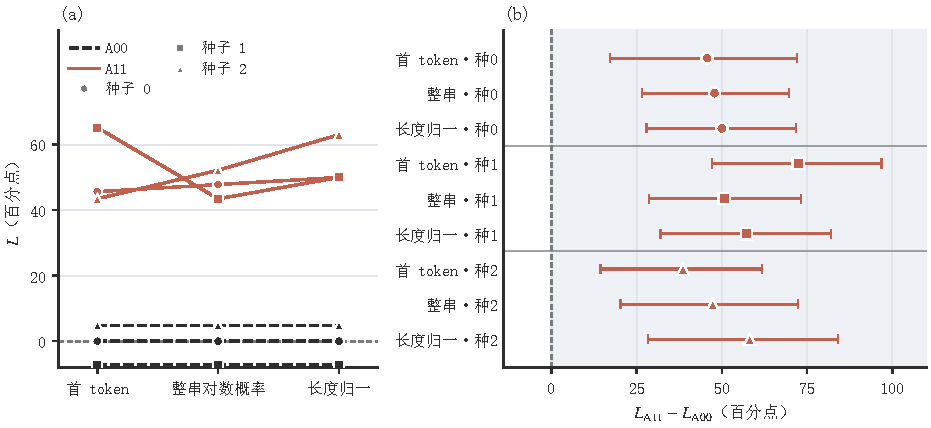
\includegraphics[width=\linewidth]{figures/fig4_scoring_zh.pdf}
\caption{打分口径敏感性。(a) 两个对角单元在三种口径下的 $L$。(b) 每种口径下的版本差 $L_{\mathrm{A11}}-L_{\mathrm{A00}}$ 及其模板族区间，浅色区为正。仅对角单元做了整串打分。}
\label{fig:scoring}
\end{figure}

\subsection{行为基线}

我们也训了一个蒸馏映射器作行为基线：8 个 epoch，约 $7.34\times10^{6}$ 个可训练参数，目标是匹配接收端的原生行为；模型对与评估数据与仿射映射完全相同，但优化预算不同。它的 Self--Joint 差距在全切片上为 $1.7$ 至 $16.7$ 个百分点，若只保留四个语义切片，种子 1 的距离为 $21.7$（另两颗分别为 $15.2$、$2.2$）。也就是说，在这套数据上蒸馏基线的观测差距更小，且对切片选择敏感；如上一节所示，它的反事实误差与仿射映射并不能区分，尽管正确率相差很大。图~\ref{fig:slices} 给出按切片的分解，以及两种映射器在重建数据上的对比。

\begin{figure}[tbp]
\centering
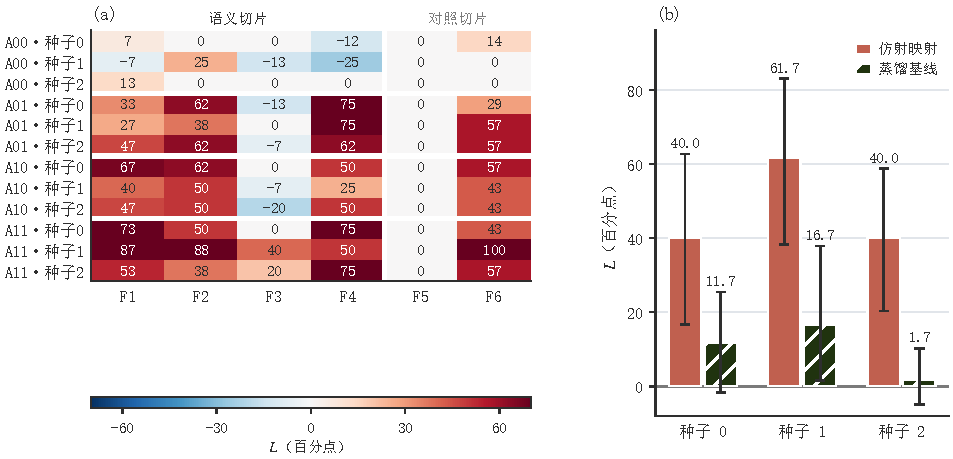
\includegraphics[width=\linewidth]{figures/fig6_slices_zh.pdf}
\caption{切片与映射器。(a) 每单元每颗种子在各切片上的 $L$（百分点）；F1--F4 为语义切片，F5 与 F6 为对照切片，不参与方向一致性分析。(b) 重建验证集上仿射映射与蒸馏基线的 $L$ 及其模板族区间；两者优化预算不同，不可直接互相当作上界。}
\label{fig:slices}
\end{figure}

\section{讨论}

\paragraph{审计改变了什么。}
校准集决定映射本身，验证集决定被测量的任务与原生参照。因此在本文的设计里，一处版本切换可以同时通过三条路径影响 $L$：迁移答案变差、原生答案变好、或两者同时发生。只报一个差值无法区分这三条路径，这也是我们把 Self 与 Joint 并列、并把“差距扩大而迁移同时变好”的例子单独写出来的原因。第二把尺子——整串打分——的作用是区分“这只是首 token 近似带来的假象”与“换一种排序方式方向仍在”；本文的结果属于后者，重建语料上的正确率损失保住了方向，但幅度有明显差异。

\paragraph{对照与指标检查如何限定这次反转。}
Joint 的反事实误差不大于无信息对照，且在一颗种子上显著更小，然而其双侧正确率坍塌；预声明的等价性检验只在三颗种子中的一颗成立。因此反事实误差不能替代迁移效用：它的尺度无法仅由 Self 分母解释，它与正确率的秩相关在两个映射器之间反号，其区间也无法区分两个正确率相差数十个百分点的映射器。并列报告原生与迁移正确率、并配上显式对照，比报告单一差距统计量更有信息量。

\paragraph{局限与下一步。}
这是一次对单一等深模型对、合成中文模板数据的审计；精确效应可能随模型对、语言、任务或校准流程而变，我们不声称跨模型或跨模型对的泛化。验证集每版本只有八个模板族、语义子集六个，区间只能算探索性。重建语料一次改变了多个属性；我们没有运行单缺陷干预（只去重、只去退化对、只做实体隔离、只做模板隔离），因此不把差距归因于泄漏或任何单一缺陷，也不声称在干净数据上存在某种机制。对角打分检查只覆盖 A00 与 A11；封存测试、第二个模型对（如 4B$\to$1.7B）以及参数量匹配的外部基线都尚未评测。早先用 SQuAD v2.0 \citep{squad18} 做的锚点在原生读者上处于地板效应，本文不把它当作证据。等价边界 $\delta=2$ 只在内部协议中预先声明，没有外部注册，等价性检验也不被认为有足够功效；失败的检验按“不确定”报告，而不推断早期的机制主张能否在重建数据上恢复。对基准审计而言，这些发现支持在解读反事实差距之前先检查语料切分与标签、并列报告原生与迁移正确率、对显式无信息对照做检验，并核对同分处理与候选打分。

\paragraph{数据与代码。}
匿名复现包内含由评估派生的数值账本、CPU 回放脚本与复现说明；它从归档的模型输出重建全部表格、套用统一同分规则并重算区间与对照检验，不需要权重或加速卡。原始模型文件以本地快照别名记录，因此快照内容的逐字节核对不在复现范围之内。

\appendix
\section{语料版本对比与对照}
\label{app:factorial}

\begin{table}[tbp]
\centering
\caption{预设的语料版本对比与交互项。估计值与样本加权的模板族区间均以百分点计；两条跨验证集的对比各自独立重采样每版本 8 个族。}
\begin{tabular}{lrrr}
\toprule
对比 & 种子 0 & 种子 1 & 种子 2\\
\midrule
\FactorialContrastRows
\bottomrule
\end{tabular}
\end{table}

\begin{table}[tbp]
\centering
\caption{族等权作为另一种估计目标（仅跨验证集的两条对比）。点估计与区间均按族等权。}
\begin{tabular}{lrrr}
\toprule
对比 & 种子 0 & 种子 1 & 种子 2\\
\midrule
\EqualFamilyRows
\bottomrule
\end{tabular}
\end{table}

\begin{table}[tbp]
\centering
\caption{仿射映射在“重建/重建”格上的首 token 偏差：族与配对两种重采样、三种对照均值，以及语义切片的方向一致率。}
\small
\begin{tabular}{lrrrrrr}
\toprule
种子 & Joint（族） & Joint（配对） & 错配 & 置零 & 随机 & 同号 / 可评估\\
\midrule
\AffineControlRows
\bottomrule
\end{tabular}
\end{table}

\begin{table}[tbp]
\centering
\caption{重建验证集上的对照均值与 Joint 对照。族 bootstrap 95\% 区间以对数概率单位计。}
\label{tab:control-mean}
\begin{tabular}{lrrr}
\toprule
种子 & 对照 & 均值 [95\% CI] & Joint [95\% CI]\\
\midrule
\ControlMeanRows
\bottomrule
\end{tabular}
\end{table}

\begin{table}[tbp]
\centering
\caption{蒸馏基线的首 token 结果。Self 与 Joint 为双侧正确率（\%），$L$ 及其区间、以及 F1--F4 的 $L$ 均为百分点。}
\small
\begin{tabular}{rrrrrr}
\toprule
种子 & Self & Joint & $L$ [区间] & F1--F4 的 $L$ & $E_{\mathrm{CF}}$ [区间]\\
\midrule
\KDRows
\bottomrule
\end{tabular}
\end{table}

A00 的 F1--F4 差距为 $0.0$、$-6.5$、$4.3$ 个百分点，其余单元在同一限制下为 $23.9$ 至 $65.2$；剔除候选相同的对照样本后，A00 为 $2.0$、$-6.1$、$4.2$，其余单元为 $28.6$ 至 $69.8$。这两项都是描述性的稳健性检查，方向上与主表一致。

\section{指标有效性与映射器区分}
\label{app:metric}

\begin{table}[tbp]
\centering
\caption{每个映射器 180 对重建验证配对上，双侧正确率与 $E_{\mathrm{CF}}$ 的 Spearman 秩相关。}
\label{tab:rank}
\begin{tabular}{lrrr}
\toprule
映射器 & $\rho$ & $p$ & 对子数\\
\midrule
\RankRows
\bottomrule
\end{tabular}
\end{table}

\begin{table}[tbp]
\centering
\caption{重建验证集上仿射映射与蒸馏基线的首 token $E_{\mathrm{CF}}$ 族区间与双侧正确率。}
\label{tab:mapper-gap}
\begin{tabular}{rrrrr}
\toprule
种子 & 仿射 $E_{\mathrm{CF}}$ & kd $E_{\mathrm{CF}}$ & 仿射 dual & kd dual\\
\midrule
\MapperGapRows
\bottomrule
\end{tabular}
\end{table}

\section{候选打分的补充敏感性}
\label{app:sequence}

\begin{table}[tbp]
\centering
\caption{整串减首 token 对 A11、以及对版本差 $L_{\mathrm{A11}}-L_{\mathrm{A00}}$ 的改动量；族等权一列改用等权估计与区间。单位均为百分点。}
\small
\begin{tabular}{rrrrr}
\toprule
& A11 & \multicolumn{3}{c}{版本差的改动量}\\
\cmidrule(lr){2-2}\cmidrule(l){3-5}
种子 & 族 & 族 & 配对 & 族等权\\
\midrule
\ScoringChangeRows
\bottomrule
\end{tabular}
\end{table}

\begin{table}[tbp]
\centering
\caption{全部 60 对验证样本上的打分敏感性。$L$ 以百分点计；该比较保留了候选相同的对照样本。}
\begin{tabular}{lrrrr}
\toprule
单元 & 种子 & 首 token & 整串 & 长度归一\\
\midrule
\AllPairsRows
\bottomrule
\end{tabular}
\end{table}

\begin{table}[tbp]
\centering
\caption{扩展的打分子集：每单元每种子保留的对子数与模板族数。保留相异候选的子集为主分析；F1--F4 与全 60 对子集为归档分数的敏感性分析。}
\label{tab:scoring-count}
\begin{tabular}{lrrrr}
\toprule
子集 & 单元 & 种子 & 对子数 & 族数\\
\midrule
\ScoringCountRows
\bottomrule
\end{tabular}
\end{table}

\begin{table}[tbp]
\centering
\caption{全部 60 对验证样本（八个模板族）上的扩展打分。$L$ 值与族 bootstrap 区间以百分点计。}
\label{tab:extended-scoring}
\begin{tabular}{lrrrr}
\toprule
单元 & 种子 & 首 token & 整串 & 长度归一\\
\midrule
\ExtendedScoringRows
\bottomrule
\end{tabular}
\end{table}

\begin{table}[tbp]
\centering
\caption{全部 60 对上的版本差 $L_{\mathrm{A11}}-L_{\mathrm{A00}}$，族 bootstrap 区间以百分点计。}
\label{tab:extended-contrast}
\begin{tabular}{rrrr}
\toprule
种子 & 首 token & 整串 & 长度归一\\
\midrule
\ExtendedContrastRows
\bottomrule
\end{tabular}
\end{table}

作为一项边界检查，把两个字符串联合分词与分别分词再拼接，在六次打分运行中给出相同的查询--候选边界；主分析子集内不存在共享首 token 的候选，也不存在一个候选是另一个真前缀的情形。每颗 A11 种子有 7 对候选长度不等；只保留等长的 39 对时，整串 $L$ 为 $48.7$、$43.6$、$56.4$ 个百分点，方向不变。等长检查是在分析阶段追加的，主比较与全 60 对比较在各自口径内使用同一批样本。

\begin{thebibliography}{9}
\bibitem[Castin et al.(2026)]{kvlingo} Castin, V., Sakamoto, K., Filippova, A., Monteiro, J., Cuturi, M., and Ablin, P. (2026). KV-Lingo: Learning KV-Cache Translators with Distillation. arXiv:2609.32610.
\bibitem[Cheng et al.(2026)]{cheng2026} Cheng, J., Das, S., and Ramnath, R. (2026). When Does Latent Communication Pay? A Causal Audit of Relayed KV Caches in Multi-Agent LLMs. arXiv:2608.04893.
\bibitem[Gardner et al.(2020)]{contrastsets} Gardner, M., Artzi, Y., Basmov, V., et al. (2020). Evaluating Models' Local Decision Boundaries via Contrast Sets. In \emph{Findings of EMNLP 2020}, 1307--1323.
\bibitem[Heo et al.(2026)]{heo2026} Heo, T., Shafipour, R., Zhao, R., Golub, M., Kamani, M. M., Borkar, R., Chandran, M. T., Zardoshti, P., and Rouhani, B. D. (2026). Cross-Model KV Cache Transfer in LLM Families: A Closed-Form Linear Mapping for Prefill Reuse. arXiv:2608.03893.
\bibitem[Kapoor and Narayanan(2023)]{kapoor2023} Kapoor, S. and Narayanan, A. (2023). Leakage and the Reproducibility Crisis in Machine-Learning-Based Science. \emph{Patterns}, 4(9):100804.
\bibitem[Qiu et al.(2026)]{cachelink} Qiu, H., Tang, Y., Song, Z., Han, R., Qiao, Z., and Zhang, M. (2026). CacheLink: Functional KV Transport for Zero-Prefill Cross-Model Context Handoff. arXiv:2610.15509.
\bibitem[Rajpurkar et al.(2018)]{squad18} Rajpurkar, P., Jia, R., and Liang, P. (2018). Know What You Don't Know: Unanswerable Questions for SQuAD. In \emph{ACL 2018 (Short Papers)}, 784--789.
\end{thebibliography}

\end{document}
